% \begin{document}

\usetikzlibrary{arrows.meta} % For double arrows

\chapter{Dropbox}

TLA+ is a \textit{thinking tool}. Writing a specification with TLA+ and verify
it against the model checker encourages the designer to exhaustively consider
all corner cases in the design. In this chapter, we will specify a Dropbox-like
service with TLA+ and use the model checker to flesh out the design.\\

\section{Design}

The simplified Dropbox-like service includes a block server that holds physical 
copies of all versions of user files, and a meta server that holds meta data on
all the files and path to the block server. A client contacts both meta and
block server as needed to keep up-to-date. In this design, client attempts to
stay up-to-date on all the file meta, but selectively download the physical
files as needed to save bandwidth.\\

A client can make local changes to a file. The updated file is committed when
the client syncs with meta and block server. The change is then propagated to
the other clients. If multiple clients made changes to the same file, the first
one to upload wins and the other clients need to rebase their changes on top of
latest and attempt to upload again.\\

The system design is visualized below:\\

\begin{center}
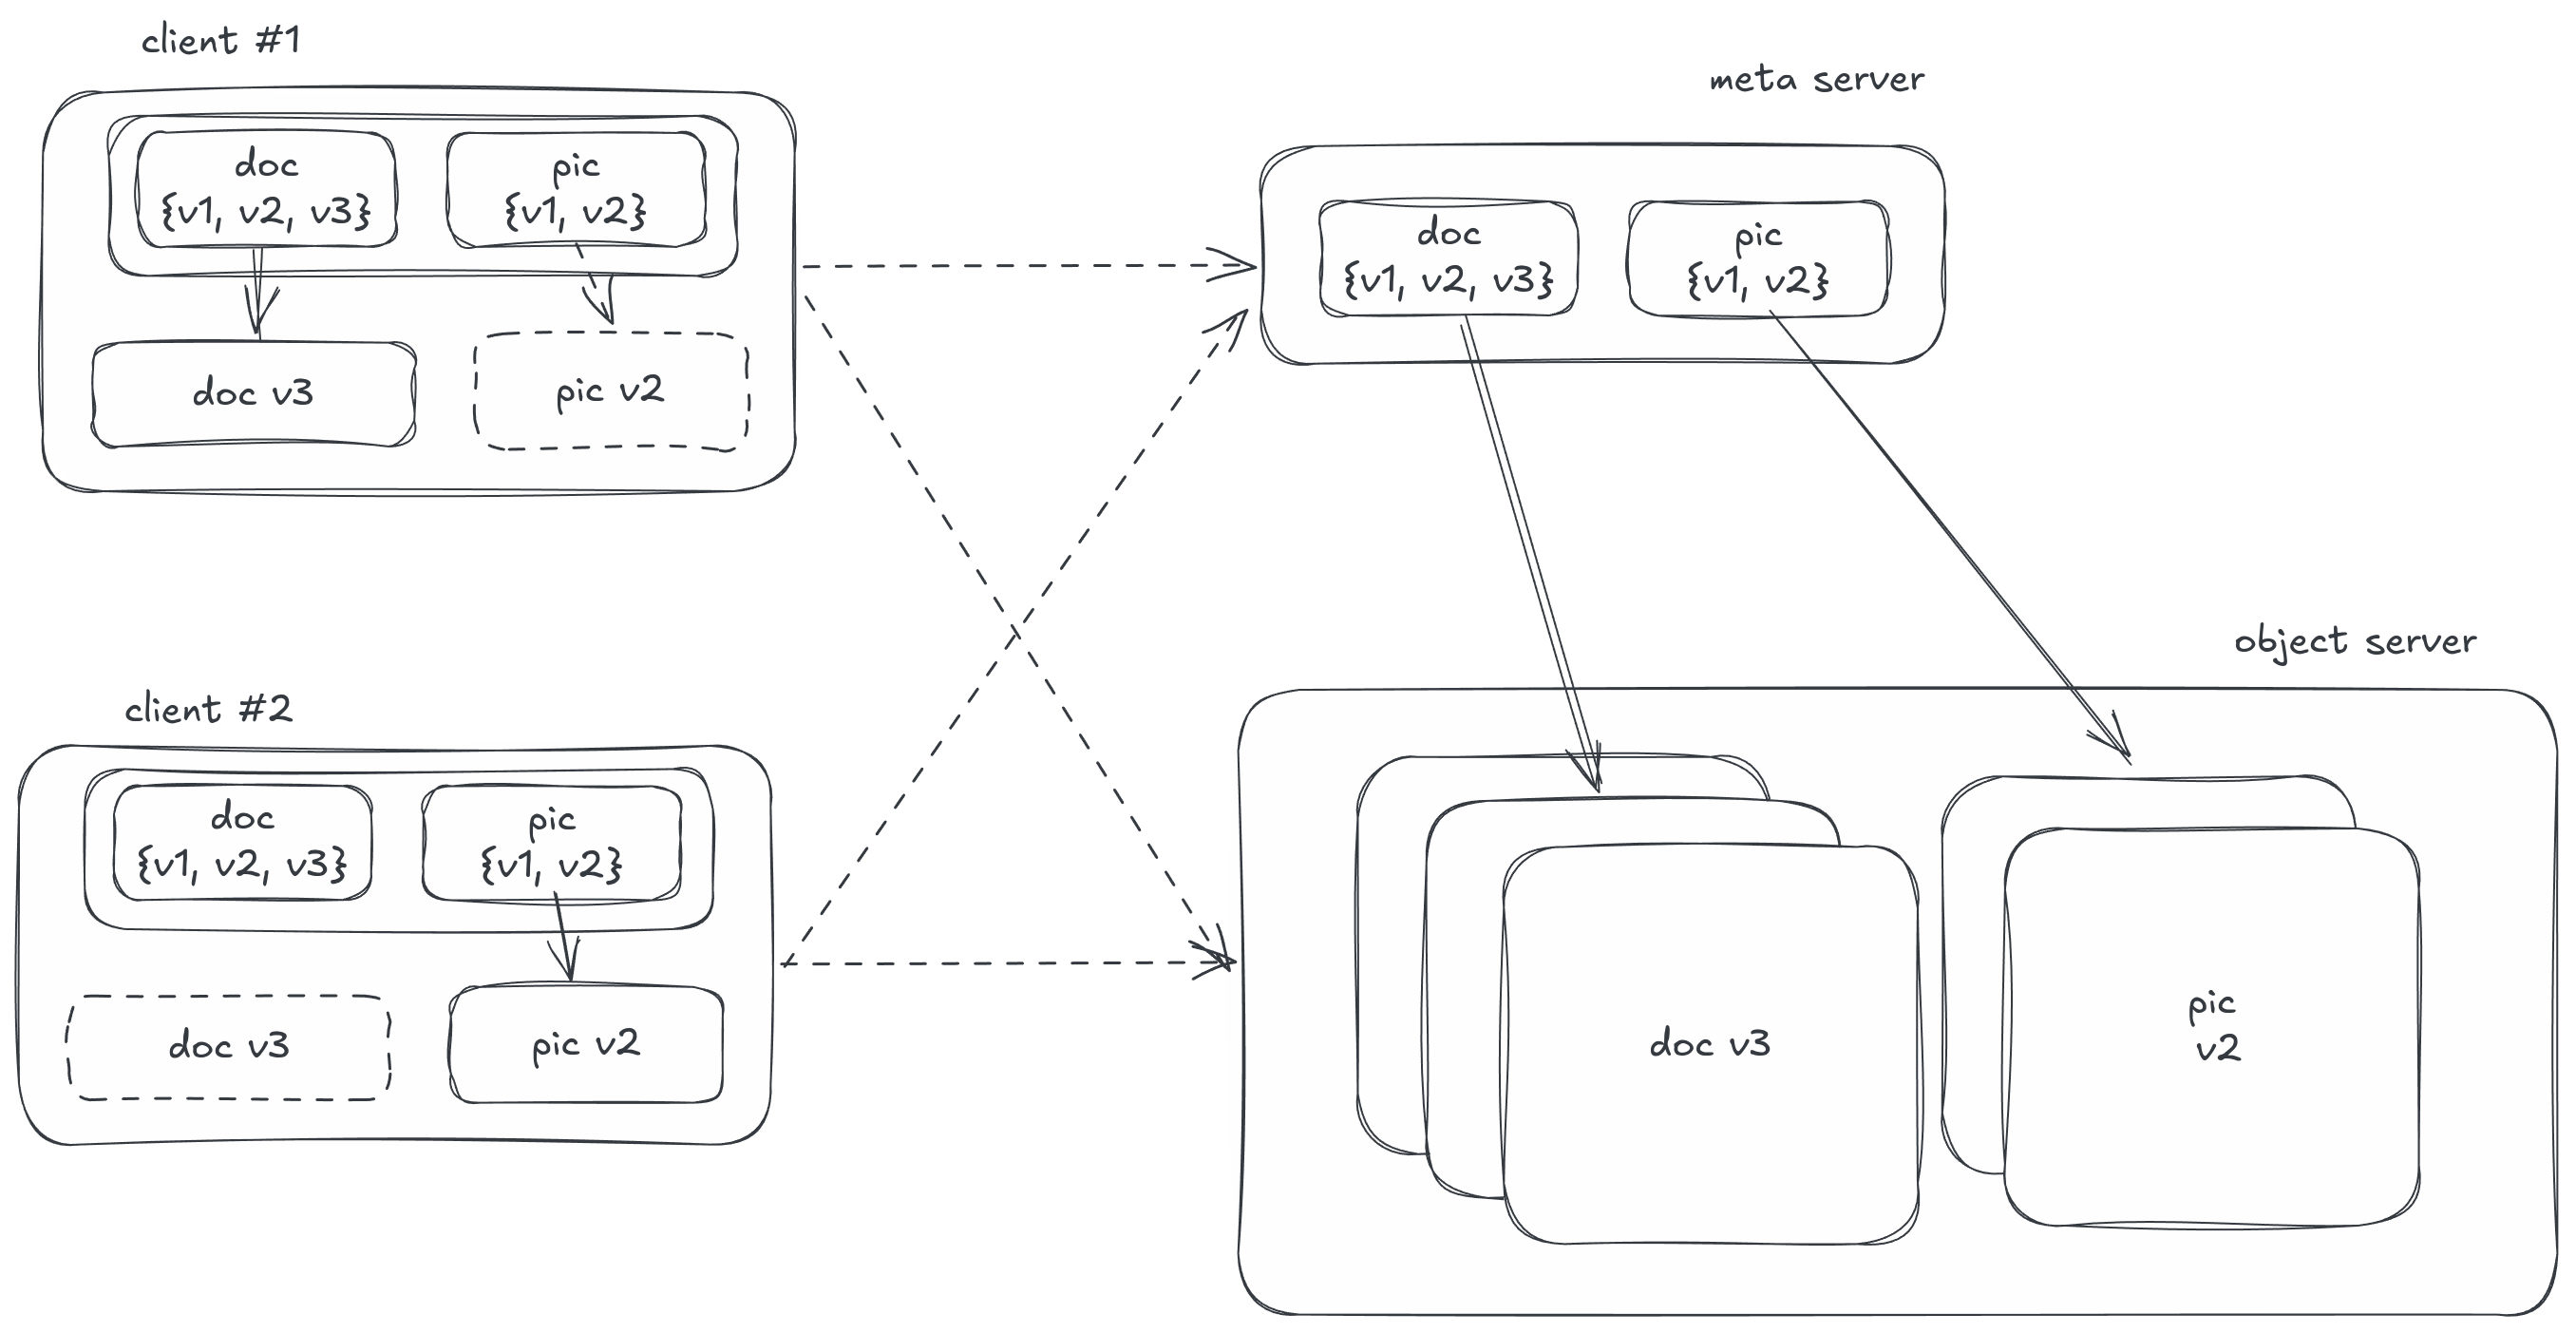
\includegraphics[width=300pt]{dropbox}
\end{center}

\section{Spec}

The following describes the variables used track system state:\\
\begin{tla}
Init ==
    /\ meta_server = [f \in Files |-> {1}]                 
    /\ block_server = [f \in Files |-> <<5>>]
    /\ client_meta = [k \in Clients |-> meta_server]
    /\ client_change = [k \in Clients |-> [f \in Files |-> FALSE]]
    /\ client_block = [k \in Clients |-> <<>>]
\end{tla}
\begin{tlatex}
\@x{ Init \.{\defeq}}%
 \@x{\@s{16.4} \.{\land} meta\_server \.{=} [ f \.{\in} Files \.{\mapsto} \{ 1
 \} ]}%
 \@x{\@s{16.4} \.{\land} block\_server \.{=} [ f \.{\in} Files \.{\mapsto}
 {\langle} 5 {\rangle} ]}%
 \@x{\@s{16.4} \.{\land} client\_meta \.{=} [ k \.{\in} Clients \.{\mapsto}
 meta\_server ]}%
 \@x{\@s{16.4} \.{\land} client\_change \.{=} [ k \.{\in} Clients \.{\mapsto}
 [ f \.{\in} Files \.{\mapsto} {\FALSE} ] ]}%
 \@x{\@s{16.4} \.{\land} client\_block \.{=} [ k \.{\in} Clients \.{\mapsto}
 {\langle} {\rangle} ]}%
\end{tlatex}

\begin{itemize}
    \item \textit{meta\_server} is a lookup table of filename to a set of revisions.
    \item \textit{block\_server} is a lookup table of filename to a list of sizes, ordered by revision.
    \item \textit{client\_meta} represents client's local copy of the file meta.
    \item \textit{client\_block} is client's block storage, only holding version of the file specified by client meta.
    \item \textit{client\_change} is a per client per file lookup tracking if the file has been changed locally.
\end{itemize}

To paint a more concrete picture, this is a snapshot of a state:
\begin{verbatim}
State 94375:
/\ client_block = [c0 |-> [f0 |-> 9, f1 |-> 5], 
                   c1 |-> [f0 |-> 9]]
/\ client_meta = [c0 |-> [f0 |-> 4, f1 |-> 2], 
                  c1 |-> [f0 |-> 2, f1 |-> 1]]
/\ block_server = [f0 |-> <<5, 5, 7>>, f1 |-> <<5, 5>>]
/\ meta_server = [f0 |-> 3, f1 |-> 2]
/\ client_change = [c0 |-> [f0 |-> TRUE, f1 |-> FALSE], 
                    c1 |-> [f0 |-> TRUE, f1 |-> FALSE]]
\end{verbatim}

In this state:
\begin{itemize}
    \item The meta and block server have 2 files: File 0 has 3 revisions and file 1 has 2.
    \item Client 0 downloaded both file 0 and 1.
    \item Client 0 modified file 0 (bumped the revision to 4) but did not modify file 1.
    \item Client 1 meta is out-of-date on both file 0 and 1, but modified file 0.
    \item Client 1 has only downloaded the older revision of file 1, but also modified it.
\end{itemize}

The set of actions allowed is defined below:\\
\begin{tla}
Next ==
    \/ \E k \in Clients: 
        \E f \in Files: 
            \/ SyncMeta(k, f)
            \/ Download(k, f)
            \/ Modify(k, f)
            \/ Upload(k, f)
\end{tla}
\begin{tlatex}
\@x{ Next \.{\defeq}}%
\@x{\@s{16.4} \.{\lor} \E\, k \.{\in} Clients \.{:}}%
\@x{\@s{20.5} \E\, f \.{\in} Files \.{:}}%
\@x{\@s{24.6} \.{\lor} SyncMeta ( k ,\, f )}%
\@x{\@s{24.6} \.{\lor} Download ( k ,\, f )}%
\@x{\@s{24.6} \.{\lor} Modify ( k ,\, f )}%
\@x{\@s{24.6} \.{\lor} Upload ( k ,\, f )}%
\end{tlatex}
\\

In every state, the system can choose to synchronize meta of a file, download a
file, modify a file, or upload a changed file. Some of these operations depend
on each other. For example, a file can only be modified if it has been
downloaded.\\ 

Let us first take a look at \textit{SyncMeta}:\\

\begin{tla}
TailIndex(s) ==
    MaxS(DOMAIN s)

SyncObject(k, f) == 
    IF f \in DOMAIN client_block[k] THEN 
        client_block' 
            = [client_block EXCEPT ![k] 
                = [client_block[k] EXCEPT ![f]
                    = block_server[f][TailIndex(block_server[f])]]]
    ELSE 
        UNCHANGED client_block

SyncMeta(k, f) == 
    IF client_meta[k][f] < meta_server[f]
    \/ (client_meta[k][f] = meta_server[f] /\ client_change[k][f]) THEN 
        \* sync client meta
        /\ client_meta' 
            = [client_meta EXCEPT ![k] 
                = [client_meta[k] EXCEPT ![f]
                    = meta_server[f]]]
        \* sync downloaded file
        /\ SyncObject(k, f)
        /\ client_change' 
            = [client_change EXCEPT ![k] 
                = [client_change[k] EXCEPT ![f] = FALSE]]
        /\ UNCHANGED <<meta_server, block_server>>
    ELSE 
        /\ UNCHANGED vars
\end{tla}
\begin{tlatex}
\@x{ TailIndex ( s ) \.{\defeq}}%
\@x{\@s{16.4} MaxS ( {\DOMAIN} s )}%
\@pvspace{8.0pt}%
\@x{ SyncObject ( k ,\, f ) \.{\defeq}}%
\@x{\@s{16.4} {\IF} f \.{\in} {\DOMAIN} client\_block [ k ] \.{\THEN}}%
\@x{\@s{20.5} client\_block \.{'}}%
\@x{\@s{36.9} \.{=} [ client\_block {\EXCEPT} {\bang} [ k ]}%
\@x{\@s{41.0} \.{=} [ client\_block [ k ] {\EXCEPT} {\bang} [ f ]}%
 \@x{\@s{45.1} \.{=} block\_server [ f ] [ TailIndex ( block\_server [ f ] ) ]
 ] ]}%
\@x{\@s{16.4} \.{\ELSE}}%
\@x{\@s{32.8} {\UNCHANGED} client\_block}%
\@pvspace{8.0pt}%
\@x{ SyncMeta ( k ,\, f ) \.{\defeq}}%
\@x{\@s{16.4} {\IF} client\_meta [ k ] [ f ] \.{<} meta\_server [ f ]}%
 \@x{\@s{16.4} \.{\lor} ( client\_meta [ k ] [ f ] \.{=} meta\_server [ f ]
 \.{\land} client\_change [ k ] [ f ] ) \.{\THEN}}%
\@x{\@s{16.4}}%
\@y{%
  sync client meta
}%
\@xx{}%
\@x{\@s{16.4} \.{\land} client\_meta \.{'}}%
\@x{\@s{20.5} \.{=} [ client\_meta {\EXCEPT} {\bang} [ k ]}%
\@x{\@s{24.6} \.{=} [ client\_meta [ k ] {\EXCEPT} {\bang} [ f ]}%
\@x{\@s{28.7} \.{=} meta\_server [ f ] ] ]}%
\@x{\@s{16.4}}%
\@y{%
  sync downloaded file
}%
\@xx{}%
\@x{\@s{16.4} \.{\land} SyncObject ( k ,\, f )}%
\@x{\@s{16.4} \.{\land} client\_change \.{'}}%
\@x{\@s{20.5} \.{=} [ client\_change {\EXCEPT} {\bang} [ k ]}%
 \@x{\@s{24.6} \.{=} [ client\_change [ k ] {\EXCEPT} {\bang} [ f ] \.{=}
 {\FALSE} ] ]}%
 \@x{\@s{16.4} \.{\land} {\UNCHANGED} {\langle} meta\_server ,\, block\_server
 {\rangle}}%
\@x{\@s{16.4} \.{\ELSE}}%
\@x{\@s{32.8} \.{\land} {\UNCHANGED} vars}%
\end{tlatex}
\\

The client syncs with remote when it is out-of-date. This happens when: remote
has higher revision of the file, or if the client has the same revision of the
file but \textit{local\_change} is set. The current implementation discards and
force update to remote. Practically, the client should rebase and resolve the
conflict.\\

\textit{SyncObject} resets the file to match the remote. This is done by getting
the size of the latest revision for the file. TLA+ doesn't natively provide a
function to get the last element, so \textit{TailIndex} function was added to
facilitate this.\\

The following defines \textit{Download}:\\
\begin{tla}
Download(k, f) == 
    \* only download if meta is up-to-date with no local changes
    /\ client_change[k][f] = FALSE
    /\ client_meta[k][f] = meta_server[f]
    \* Download the latest version
    /\ client_block'
        = [client_block EXCEPT ![k] 
            = [ff \in DOMAIN client_block[k] \cup {f} 
                |-> IF ff # f 
                    THEN client_block[k][ff] 
                    ELSE block_server[f][MaxS(DOMAIN block_server[f])]]]
    /\ UNCHANGED <<client_change, client_meta, meta_server, block_server>>
\end{tla}
\begin{tlatex}
\@x{ Download ( k ,\, f ) \.{\defeq}}%
\@x{\@s{16.4}}%
\@y{%
  only download if meta is up-to-date with no local changes
}%
\@xx{}%
\@x{\@s{16.4} \.{\land} client\_change [ k ] [ f ] \.{=} {\FALSE}}%
\@x{\@s{16.4} \.{\land} client\_meta [ k ] [ f ] \.{=} meta\_server [ f ]}%
\@x{\@s{16.4}}%
\@y{%
  Download the latest version
}%
\@xx{}%
\@x{\@s{16.4} \.{\land} client\_block \.{'}}%
\@x{\@s{20.5} \.{=} [ client\_block {\EXCEPT} {\bang} [ k ]}%
 \@x{\@s{24.6} \.{=} [ ff \.{\in} {\DOMAIN} client\_block [ k ] \.{\cup} \{ f
 \}}%
\@x{\@s{28.7} \.{\mapsto} {\IF} ff \.{\neq} f}%
\@x{\@s{28.7} \.{\THEN} client\_block [ k ] [ ff ]}%
 \@x{\@s{28.7} \.{\ELSE} block\_server [ f ] [ MaxS ( {\DOMAIN} block\_server
 [ f ] ) ] ] ]}%
 \@x{\@s{16.4} \.{\land} {\UNCHANGED} {\langle} client\_change ,\,
 client\_meta ,\, meta\_server ,\, block\_server {\rangle}}%
\end{tlatex}
\\

The client only downloads if file meta is up-to-date and has not been modified
locally.\\

The \textit{Modify} function is defined below:\\

\begin{tla}
Modify(k, f) ==
    /\ client_change[k][f] = FALSE
    \* add new version to client meta
    /\ client_meta' 
        = [client_meta EXCEPT ![k] 
            = [client_meta[k] EXCEPT ![f] 
                = client_meta[k][f] + 1]]
    \* bump client block
    /\ f \in DOMAIN client_block[k]
    /\ \E s \in Sizes: 
       client_block'
        = [client_block EXCEPT ![k] 
            = [client_block[k] EXCEPT ![f] = s]]
    /\ client_change' 
        = [client_change EXCEPT ![k] 
            = [client_change[k] EXCEPT ![f] = TRUE]]
    /\ UNCHANGED <<meta_server, block_server>>
\end{tla}
\begin{tlatex}
\@x{ Modify ( k ,\, f ) \.{\defeq}}%
\@x{\@s{16.4} \.{\land} client\_change [ k ] [ f ] \.{=} {\FALSE}}%
\@x{\@s{16.4}}%
\@y{%
  add new version to client meta
}%
\@xx{}%
\@x{\@s{16.4} \.{\land} client\_meta \.{'}}%
\@x{\@s{20.5} \.{=} [ client\_meta {\EXCEPT} {\bang} [ k ]}%
\@x{\@s{24.6} \.{=} [ client\_meta [ k ] {\EXCEPT} {\bang} [ f ]}%
\@x{\@s{28.7} \.{=} client\_meta [ k ] [ f ] \.{+} 1 ] ]}%
\@x{\@s{16.4}}%
\@y{%
  bump client block
}%
\@xx{}%
\@x{\@s{16.4} \.{\land} f \.{\in} {\DOMAIN} client\_block [ k ]}%
\@x{\@s{16.4} \.{\land} \E\, s \.{\in} Sizes \.{:}}%
\@x{\@s{16.4} client\_block \.{'}}%
\@x{\@s{20.5} \.{=} [ client\_block {\EXCEPT} {\bang} [ k ]}%
 \@x{\@s{24.6} \.{=} [ client\_block [ k ] {\EXCEPT} {\bang} [ f ] \.{=} s ]
 ]}%
\@x{\@s{16.4} \.{\land} client\_change \.{'}}%
\@x{\@s{20.5} \.{=} [ client\_change {\EXCEPT} {\bang} [ k ]}%
 \@x{\@s{24.6} \.{=} [ client\_change [ k ] {\EXCEPT} {\bang} [ f ] \.{=}
 {\TRUE} ] ]}%
 \@x{\@s{16.4} \.{\land} {\UNCHANGED} {\langle} meta\_server ,\, block\_server
 {\rangle}}%
\end{tlatex}
\\

A file can only be modified if it hasn't been. While the client can modify a 
file multiple times, this is modeled as a single revision until the file is
uploaded to remote. A new version of the file is created by bumping the client
local file meta, mark file as changed and assign the file a random size using
existential qualifier.\\

Finally, let's take a look at \textit{Upload}:\\

\begin{tla}
Upload(k, f) == 
    \* client is ahead of the remote with local change
    /\ meta_server[f] < client_meta[k][f]
    /\ client_change[k][f]
    /\ meta_server' 
        = [meta_server EXCEPT ![f] 
            = client_meta[k][f]] \* upload our version
    /\ block_server' = [block_server EXCEPT ![f] 
                        = Append(block_server[f], client_block[k][f])]
    /\ client_change' 
        = [client_change EXCEPT ![k] 
            = [client_change[k] EXCEPT ![f] = FALSE]]
    /\ UNCHANGED <<client_block, client_meta>>
\end{tla}
\begin{tlatex}
\@x{ Upload ( k ,\, f ) \.{\defeq}}%
\@x{\@s{16.4}}%
\@y{%
  client is ahead of the remote with local change
}%
\@xx{}%
\@x{\@s{16.4} \.{\land} meta\_server [ f ] \.{<} client\_meta [ k ] [ f ]}%
\@x{\@s{16.4} \.{\land} client\_change [ k ] [ f ]}%
\@x{\@s{16.4} \.{\land} meta\_server \.{'}}%
\@x{\@s{20.5} \.{=} [ meta\_server {\EXCEPT} {\bang} [ f ]}%
\@x{\@s{24.6} \.{=} client\_meta [ k ] [ f ] ]}%
\@y{%
  upload our version
}%
\@xx{}%
 \@x{\@s{16.4} \.{\land} block\_server \.{'} \.{=} [ block\_server {\EXCEPT}
 {\bang} [ f ]}%
 \@x{\@s{16.4} \.{=} Append ( block\_server [ f ] ,\, client\_block [ k ] [ f
 ] ) ]}%
\@x{\@s{16.4} \.{\land} client\_change \.{'}}%
\@x{\@s{20.5} \.{=} [ client\_change {\EXCEPT} {\bang} [ k ]}%
 \@x{\@s{24.6} \.{=} [ client\_change [ k ] {\EXCEPT} {\bang} [ f ] \.{=}
 {\FALSE} ] ]}%
 \@x{\@s{16.4} \.{\land} {\UNCHANGED} {\langle} client\_block ,\, client\_meta
 {\rangle}}%
\end{tlatex}
\\

Client uploads when it is ahead of remote and has local changes. If the client
is not ahead of remote, remote may have newer version of the file. In such case 
client will call \textit{SyncMeta} to synchronize the remote.

\section{Safety}

\section{Liveness}

% \end{document}

